% Options for packages loaded elsewhere

\PassOptionsToPackage{unicode}{hyperref}
\PassOptionsToPackage{hyphens}{url}
%
\documentclass[
]{article}
\usepackage[english,russian]{babel}
\usepackage{amsmath,amssymb}
\usepackage{lmodern}
\usepackage{iftex}
\ifPDFTeX
  \usepackage[T1]{fontenc}
  \usepackage[utf8]{inputenc}
  \usepackage{textcomp} % provide euro and other symbols
\else % if luatex or xetex
  \usepackage{unicode-math}
  \defaultfontfeatures{Scale=MatchLowercase}
  \defaultfontfeatures[\rmfamily]{Ligatures=TeX,Scale=1}
\fi
% Use upquote if available, for straight quotes in verbatim environments
\IfFileExists{upquote.sty}{\usepackage{upquote}}{}
\IfFileExists{microtype.sty}{% use microtype if available
  \usepackage[]{microtype}
  \UseMicrotypeSet[protrusion]{basicmath} % disable protrusion for tt fonts
}{}
\makeatletter
\@ifundefined{KOMAClassName}{% if non-KOMA class
  \IfFileExists{parskip.sty}{%
    \usepackage{parskip}
  }{% else
    \setlength{\parindent}{0pt}
    \setlength{\parskip}{6pt plus 2pt minus 1pt}}
}{% if KOMA class
  \KOMAoptions{parskip=half}}
\makeatother
\usepackage{xcolor}
\IfFileExists{xurl.sty}{\usepackage{xurl}}{} % add URL line breaks if available
\IfFileExists{bookmark.sty}{\usepackage{bookmark}}{\usepackage{hyperref}}
\hypersetup{
  pdflang={ru-RU},
  hidelinks,
  pdfcreator={LaTeX via pandoc}}
\urlstyle{same} % disable monospaced font for URLs
\usepackage[margin=1in]{geometry}
\usepackage{color}
\usepackage{fancyvrb}
\newcommand{\VerbBar}{|}
\newcommand{\VERB}{\Verb[commandchars=\\\{\}]}
\DefineVerbatimEnvironment{Highlighting}{Verbatim}{commandchars=\\\{\}}
% Add ',fontsize=\small' for more characters per line
\usepackage{framed}
\definecolor{shadecolor}{RGB}{248,248,248}
\newenvironment{Shaded}{\begin{snugshade}}{\end{snugshade}}
\newcommand{\AlertTok}[1]{\textcolor[rgb]{0.94,0.16,0.16}{#1}}
\newcommand{\AnnotationTok}[1]{\textcolor[rgb]{0.56,0.35,0.01}{\textbf{\textit{#1}}}}
\newcommand{\AttributeTok}[1]{\textcolor[rgb]{0.77,0.63,0.00}{#1}}
\newcommand{\BaseNTok}[1]{\textcolor[rgb]{0.00,0.00,0.81}{#1}}
\newcommand{\BuiltInTok}[1]{#1}
\newcommand{\CharTok}[1]{\textcolor[rgb]{0.31,0.60,0.02}{#1}}
\newcommand{\CommentTok}[1]{\textcolor[rgb]{0.56,0.35,0.01}{\textit{#1}}}
\newcommand{\CommentVarTok}[1]{\textcolor[rgb]{0.56,0.35,0.01}{\textbf{\textit{#1}}}}
\newcommand{\ConstantTok}[1]{\textcolor[rgb]{0.00,0.00,0.00}{#1}}
\newcommand{\ControlFlowTok}[1]{\textcolor[rgb]{0.13,0.29,0.53}{\textbf{#1}}}
\newcommand{\DataTypeTok}[1]{\textcolor[rgb]{0.13,0.29,0.53}{#1}}
\newcommand{\DecValTok}[1]{\textcolor[rgb]{0.00,0.00,0.81}{#1}}
\newcommand{\DocumentationTok}[1]{\textcolor[rgb]{0.56,0.35,0.01}{\textbf{\textit{#1}}}}
\newcommand{\ErrorTok}[1]{\textcolor[rgb]{0.64,0.00,0.00}{\textbf{#1}}}
\newcommand{\ExtensionTok}[1]{#1}
\newcommand{\FloatTok}[1]{\textcolor[rgb]{0.00,0.00,0.81}{#1}}
\newcommand{\FunctionTok}[1]{\textcolor[rgb]{0.00,0.00,0.00}{#1}}
\newcommand{\ImportTok}[1]{#1}
\newcommand{\InformationTok}[1]{\textcolor[rgb]{0.56,0.35,0.01}{\textbf{\textit{#1}}}}
\newcommand{\KeywordTok}[1]{\textcolor[rgb]{0.13,0.29,0.53}{\textbf{#1}}}
\newcommand{\NormalTok}[1]{#1}
\newcommand{\OperatorTok}[1]{\textcolor[rgb]{0.81,0.36,0.00}{\textbf{#1}}}
\newcommand{\OtherTok}[1]{\textcolor[rgb]{0.56,0.35,0.01}{#1}}
\newcommand{\PreprocessorTok}[1]{\textcolor[rgb]{0.56,0.35,0.01}{\textit{#1}}}
\newcommand{\RegionMarkerTok}[1]{#1}
\newcommand{\SpecialCharTok}[1]{\textcolor[rgb]{0.00,0.00,0.00}{#1}}
\newcommand{\SpecialStringTok}[1]{\textcolor[rgb]{0.31,0.60,0.02}{#1}}
\newcommand{\StringTok}[1]{\textcolor[rgb]{0.31,0.60,0.02}{#1}}
\newcommand{\VariableTok}[1]{\textcolor[rgb]{0.00,0.00,0.00}{#1}}
\newcommand{\VerbatimStringTok}[1]{\textcolor[rgb]{0.31,0.60,0.02}{#1}}
\newcommand{\WarningTok}[1]{\textcolor[rgb]{0.56,0.35,0.01}{\textbf{\textit{#1}}}}
\usepackage{graphicx}
\makeatletter
\def\maxwidth{\ifdim\Gin@nat@width>\linewidth\linewidth\else\Gin@nat@width\fi}
\def\maxheight{\ifdim\Gin@nat@height>\textheight\textheight\else\Gin@nat@height\fi}
\makeatother
% Scale images if necessary, so that they will not overflow the page
% margins by default, and it is still possible to overwrite the defaults
% using explicit options in \includegraphics[width, height, ...]{}
\setkeys{Gin}{width=\maxwidth,height=\maxheight,keepaspectratio}
% Set default figure placement to htbp
\makeatletter
\def\fps@figure{htbp}
\makeatother
\setlength{\emergencystretch}{3em} % prevent overfull lines
\providecommand{\tightlist}{%
  \setlength{\itemsep}{0pt}\setlength{\parskip}{0pt}}
\setcounter{secnumdepth}{-\maxdimen} % remove section numbering
\ifLuaTeX
\usepackage[bidi=basic]{babel}
\else
\usepackage[bidi=default]{babel}
\fi
\babelprovide[main,import]{russian}
% get rid of language-specific shorthands (see #6817):
\let\LanguageShortHands\languageshorthands
\def\languageshorthands#1{}
\ifLuaTeX
  \usepackage{selnolig}  % disable illegal ligatures
\fi

\author{}
\date{\vspace{-2.5em}}

\begin{document}

\begin{Shaded}
\begin{Highlighting}[]
  \FunctionTok{library}\NormalTok{(}\StringTok{"svd"}\NormalTok{)}
  \FunctionTok{library}\NormalTok{(}\StringTok{"forecast"}\NormalTok{)}
  \FunctionTok{library}\NormalTok{(}\StringTok{"Rssa"}\NormalTok{)}
  \FunctionTok{library}\NormalTok{(}\StringTok{"lattice"}\NormalTok{)}
  \FunctionTok{library}\NormalTok{(}\StringTok{"knitr"}\NormalTok{)}
\end{Highlighting}
\end{Shaded}

\hypertarget{i.-ux441ux43eux437ux434ux430ux43dux438ux435-ux432ux440ux435ux43cux435ux43dux43dux43eux433ux43e-ux440ux44fux434ux430-ux434ux43bux44f-ux43fux440ux438ux43cux435ux43dux435ux43dux438ux44f-ux430ux43bux433ux43eux440ux438ux442ux43cux430}{%
\section{I. Создание временного ряда для применения
алгоритма}\label{i.-ux441ux43eux437ux434ux430ux43dux438ux435-ux432ux440ux435ux43cux435ux43dux43dux43eux433ux43e-ux440ux44fux434ux430-ux434ux43bux44f-ux43fux440ux438ux43cux435ux43dux435ux43dux438ux44f-ux430ux43bux433ux43eux440ux438ux442ux43cux430}}

\begin{Shaded}
\begin{Highlighting}[]
\NormalTok{  trend\_function1 }\OtherTok{\textless{}{-}} \ControlFlowTok{function}\NormalTok{(n)\{}
    \CommentTok{\# Input: аргумент {-} отметка на временной оси}
    \CommentTok{\# Output: значение тренда как функции в точке}
    \FunctionTok{return}\NormalTok{ (}\FloatTok{0.08} \SpecialCharTok{*} \FunctionTok{exp}\NormalTok{(}\FloatTok{0.01} \SpecialCharTok{*}\NormalTok{ n))}
\NormalTok{  \}}
\end{Highlighting}
\end{Shaded}

\begin{Shaded}
\begin{Highlighting}[]
\NormalTok{  harmonic\_component1\_function }\OtherTok{\textless{}{-}} \ControlFlowTok{function}\NormalTok{(n)\{}
    \CommentTok{\# Input: аргумент {-} отметка на временной оси}
    \CommentTok{\# Output: значение гармонической компоненты как функции в точке}
    \FunctionTok{return}\NormalTok{ (}\FloatTok{0.25} \SpecialCharTok{*} \FunctionTok{cos}\NormalTok{(}\DecValTok{2} \SpecialCharTok{*}\NormalTok{ pi }\SpecialCharTok{*}\NormalTok{ n }\SpecialCharTok{/} \DecValTok{8} \SpecialCharTok{+}\NormalTok{ pi }\SpecialCharTok{/} \DecValTok{4}\NormalTok{)) }
\NormalTok{  \}}
\end{Highlighting}
\end{Shaded}

\begin{Shaded}
\begin{Highlighting}[]
\NormalTok{  harmonic\_component2\_function }\OtherTok{\textless{}{-}} \ControlFlowTok{function}\NormalTok{(n)\{}
    \CommentTok{\# Input: аргумент {-} отметка на временной оси}
    \CommentTok{\# Output: значение гармонической компоненты как функции в точке}
    \FunctionTok{return}\NormalTok{ (}\FloatTok{0.25} \SpecialCharTok{*} \FunctionTok{cos}\NormalTok{(}\DecValTok{2} \SpecialCharTok{*}\NormalTok{ pi }\SpecialCharTok{*}\NormalTok{ n }\SpecialCharTok{/} \DecValTok{3}\NormalTok{))}
\NormalTok{  \}}
\end{Highlighting}
\end{Shaded}

\begin{Shaded}
\begin{Highlighting}[]
  \FunctionTok{set.seed}\NormalTok{(}\DecValTok{11{-}10{-}2021}\NormalTok{)}
\NormalTok{  time\_series }\OtherTok{=} \DecValTok{0}\SpecialCharTok{:}\DecValTok{100}
\NormalTok{  actual\_trend }\OtherTok{\textless{}{-}} \FunctionTok{trend\_function1}\NormalTok{(time\_series)}
\NormalTok{  time\_series }\OtherTok{\textless{}{-}} \FunctionTok{trend\_function1}\NormalTok{(time\_series) }\SpecialCharTok{+} \FunctionTok{harmonic\_component1\_function}\NormalTok{(time\_series) }\SpecialCharTok{+} \FunctionTok{harmonic\_component2\_function}\NormalTok{(time\_series) }\SpecialCharTok{+} \FunctionTok{rnorm}\NormalTok{(}\DecValTok{101}\NormalTok{, }\AttributeTok{sd =} \FloatTok{0.2}\NormalTok{)}
\end{Highlighting}
\end{Shaded}

Создан временной ряд \(f_n , 0\leqslant n < N, N=101\), с функцией
тренда \(0.08e^{0.01n}\), гармониками
\(0.25 * cos(\frac{\pi n}{4} + \frac{\pi}{4})\) и
\(0.25 * cos(\frac{2 \pi n}{3})\), добавлен стандартный гауссовский шум
\(0.2 \epsilon_n\).

\begin{Shaded}
\begin{Highlighting}[]
\NormalTok{  s }\OtherTok{\textless{}{-}} \FunctionTok{ssa}\NormalTok{(time\_series, }\AttributeTok{L =} \DecValTok{48}\NormalTok{)}
  \FunctionTok{plot}\NormalTok{(s)}
\end{Highlighting}
\end{Shaded}

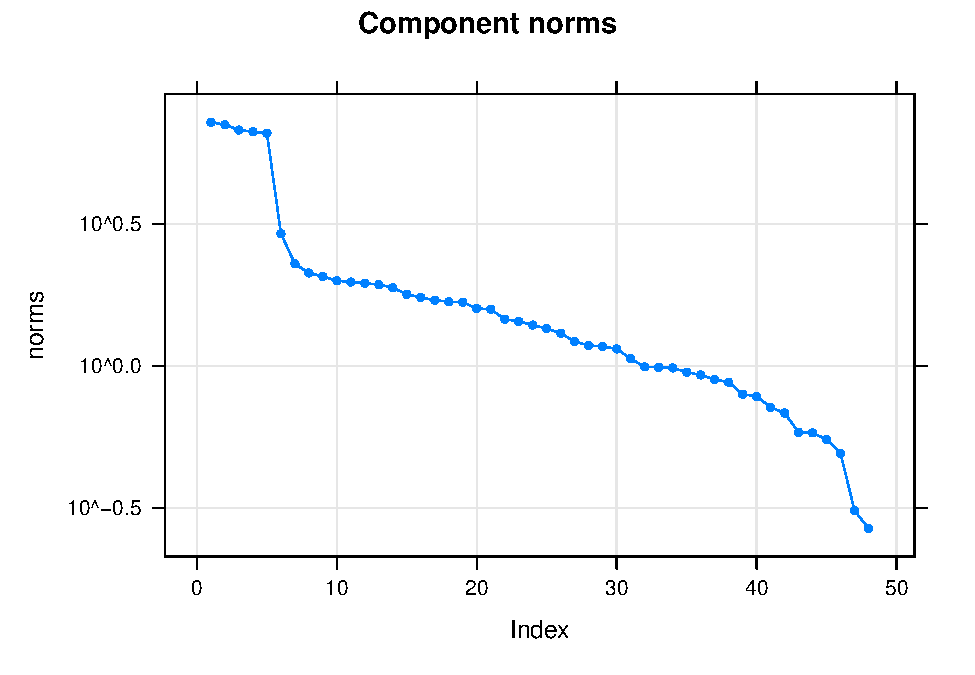
\includegraphics{eigen plot-1.pdf}

\begin{Shaded}
\begin{Highlighting}[]
\NormalTok{  grouping\_num }\OtherTok{\textless{}{-}} \DecValTok{5}
\end{Highlighting}
\end{Shaded}

\hypertarget{ii.-ux430ux432ux442ux43eux43cux430ux442ux438ux447ux435ux441ux43aux43eux435-ux432ux44bux434ux435ux43bux435ux43dux438ux435-ux442ux440ux435ux43dux434ux430}{%
\section{II. Автоматическое выделение
тренда}\label{ii.-ux430ux432ux442ux43eux43cux430ux442ux438ux447ux435ux441ux43aux43eux435-ux432ux44bux434ux435ux43bux435ux43dux438ux435-ux442ux440ux435ux43dux434ux430}}

\begin{Shaded}
\begin{Highlighting}[]
\NormalTok{  g }\OtherTok{\textless{}{-}} \FunctionTok{grouping.auto}\NormalTok{(s, }\AttributeTok{base =} \StringTok{"series"}\NormalTok{, }
                 \AttributeTok{freq.bins =} \FunctionTok{list}\NormalTok{(}\AttributeTok{Tendency =} \DecValTok{1}\SpecialCharTok{/}\DecValTok{240}\NormalTok{, }\AttributeTok{Trend =} \DecValTok{1}\SpecialCharTok{/}\DecValTok{24}\NormalTok{), }
                 \AttributeTok{threshold =} \FloatTok{0.8}\NormalTok{)}
                 
\NormalTok{  trend\_time\_series }\OtherTok{\textless{}{-}} \FunctionTok{reconstruct}\NormalTok{(s, }\AttributeTok{groups =}\NormalTok{ g)}
  
  \FunctionTok{plot}\NormalTok{(trend\_time\_series, }
   \AttributeTok{add.residuals =} \ConstantTok{FALSE}\NormalTok{, }
   \AttributeTok{plot.method =} \StringTok{"xyplot"}\NormalTok{, }\AttributeTok{superpose =} \ConstantTok{TRUE}\NormalTok{)}
\end{Highlighting}
\end{Shaded}

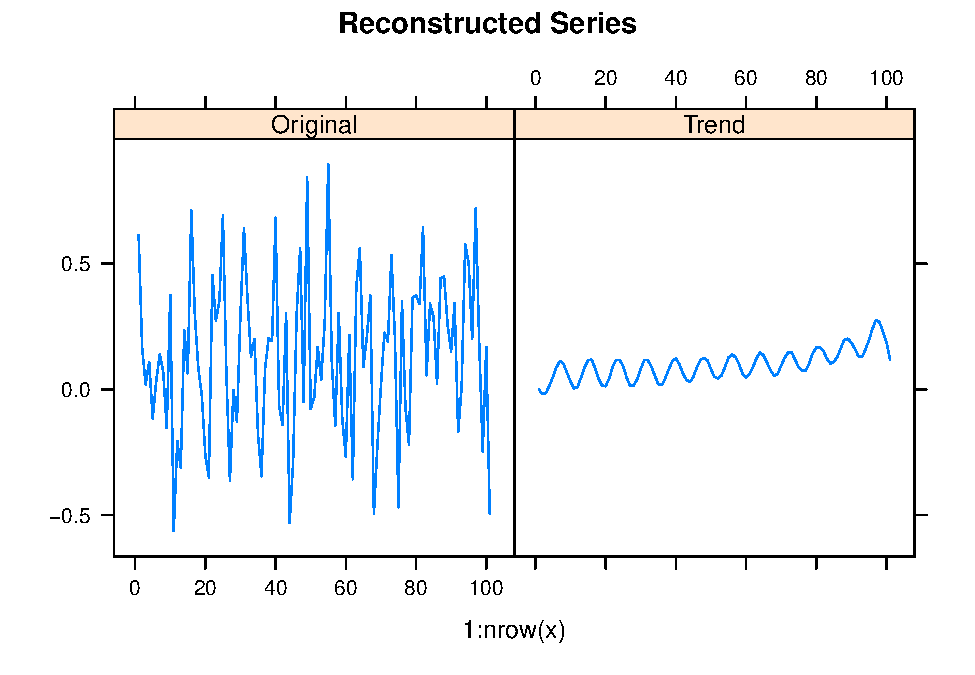
\includegraphics{decomposition-1.pdf}

\hypertarget{iii.-ux432ux44bux434ux435ux43bux435ux43dux438ux435-ux442ux440ux435ux43dux434ux430-ux441-ux43fux43eux43cux43eux449ux44cux44e-iossa}{%
\section{III. Выделение тренда с помощью
iossa}\label{iii.-ux432ux44bux434ux435ux43bux435ux43dux438ux435-ux442ux440ux435ux43dux434ux430-ux441-ux43fux43eux43cux43eux449ux44cux44e-iossa}}

\begin{Shaded}
\begin{Highlighting}[]
\NormalTok{  ioss }\OtherTok{\textless{}{-}} \FunctionTok{iossa}\NormalTok{(s, }\AttributeTok{nested.groups =} \FunctionTok{list}\NormalTok{(}\DecValTok{1}\NormalTok{, }\DecValTok{2}\NormalTok{, }\DecValTok{3}\NormalTok{, }\DecValTok{4}\NormalTok{, }\DecValTok{5}\NormalTok{))}
\NormalTok{  g\_iossa }\OtherTok{\textless{}{-}} \FunctionTok{grouping.auto}\NormalTok{(ioss, }\AttributeTok{base =} \StringTok{"series"}\NormalTok{, }
                 \AttributeTok{freq.bins =} \FunctionTok{list}\NormalTok{(}\AttributeTok{Tendency =} \DecValTok{1}\SpecialCharTok{/}\DecValTok{240}\NormalTok{, }\AttributeTok{Trend =} \DecValTok{1}\SpecialCharTok{/}\DecValTok{24}\NormalTok{), }
                 \AttributeTok{threshold =} \FloatTok{0.8}\NormalTok{)}
                 
\NormalTok{  trend\_time\_series }\OtherTok{\textless{}{-}} \FunctionTok{reconstruct}\NormalTok{(ioss, }\AttributeTok{groups =}\NormalTok{ g\_iossa)}
  
  \FunctionTok{plot}\NormalTok{(trend\_time\_series, }
   \AttributeTok{add.residuals =} \ConstantTok{FALSE}\NormalTok{, }
   \AttributeTok{plot.method =} \StringTok{"xyplot"}\NormalTok{, }\AttributeTok{superpose =} \ConstantTok{TRUE}\NormalTok{)}
\end{Highlighting}
\end{Shaded}

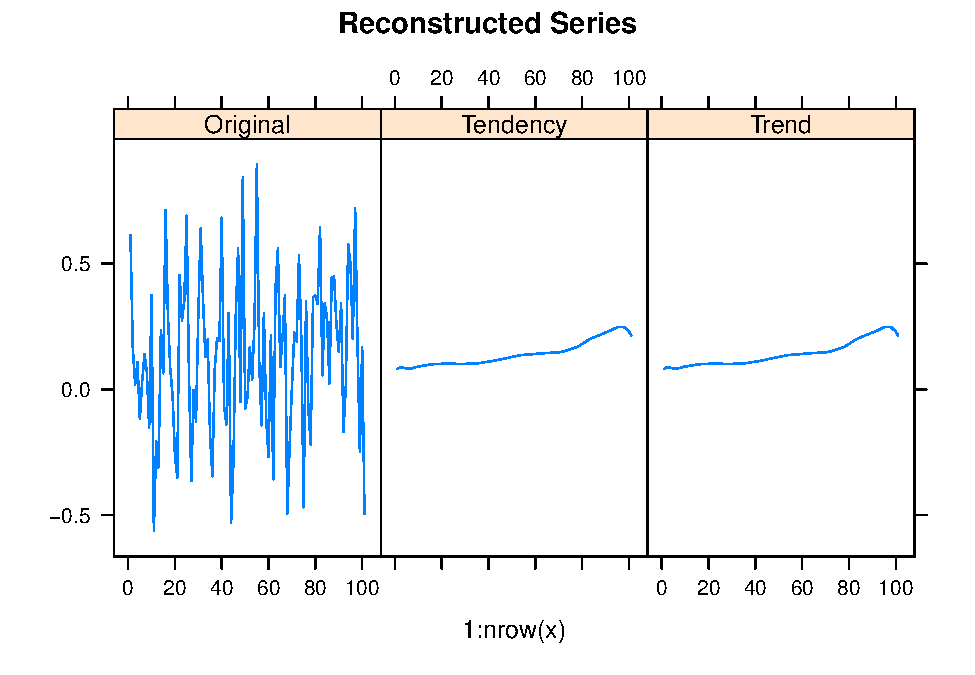
\includegraphics{iossa_trend-1.pdf}

Видно, что автоматическое выделение тренда без решения проблемы
отсутствия сильной разделимости не дало желаемого результата, тренд
смешался с гармоникой. При этом после iossa автоматическое выделение
хорошо сработало, тренд отделился от гармоник. Можно увидеть на графике
тренда экспоненту, как и было задано в начале программы. Из графика норм
собственных чисел следует, что сильной разделимости компонент сигнала
нет, поэтому после iossa можно выполнять автоматическое выделение
тренда.

\end{document}
